\documentclass[a4paper,11pt]{kth-mag}
\usepackage[T1]{fontenc}
\usepackage{textcomp}
\usepackage{lmodern}
\usepackage[utf8]{inputenc}
\usepackage[swedish,english]{babel}
\usepackage{modifications}
\usepackage{listings}
\usepackage{hyperref}
\usepackage{enumitem}
\usepackage{graphicx}
\usepackage{csquotes}
\usepackage[backend=bibtex,style=authoryear]{biblatex}
\addbibresource{references.bib}

\nonzeroparskip
\setlength{\parindent}{0pt}

\newenvironment{italicquotes}
{\begin{quote}\itshape}
{\end{quote}}

\title{Anti-analysis techniques to preserve programmer anonymity in binary
executables}

\subtitle{
    DEGREE PROJECT IN COMPUTER SCIENCE, FIRST LEVEL \\
    STOCKHOLM, SWEDEN 2016
}
\author{Johan Wikström \\ Macaully Muir}
\date{April 2016}
\blurb{
    Supervisor: Michael Schliephake \\
    Examiner: Örjan Ekeberg
}
\trita{TRITA TK: xxx yyyy-nn}
\begin{document}
\frontmatter
\pagestyle{empty}
\removepagenumbers
\maketitle
\selectlanguage{english}
\begin{abstract}
Previous research has shown that it is possible to achieve authorship
attribution with high accuracy using binary files. The idea behind authorship
attribution for binaries is that authors’ unique style will survive the
compilation process making it possible to identify the author.    

The aim of this thesis is to investigate different ways to reduce the accuracy
and see how the processing of binaries affects the author prediction accuracy.

This thesis will build on the report of Rosenblum et al. and implement the method
they used. The method uses a machine learning approach to predict the author
of the binary. The data used for prediction consists of features extracted from
the binaries. Similar to \parencite{rosenblum2011wrote} binary files used in this
thesis come from the Google Code Jam programming competition.

Results from this study indicate that compiler optimisation reduces the accuracy
achieved; however, is not enough to ensure anonymity. Using static linking
results in a more significant drop in accuracy. The data extracted shows that
optimisation and static linking results in more features that may be the cause
of the reduction in accuracy.
\end{abstract}
\clearpage
\begin{foreignabstract}{swedish}
I tidigare studier har det visat sig möjligt att med hög noggrannhet
identifiera författaren till binära filer. Idéen är att författare till kod
lämnar karaktäristiska drag i koden som går att känna igen även efter
kompilering. 

Syftet med denna rapport är att utforska olika tekniker för att minska
säkerheten då man vill bestämma vem som är författaren till binära filer och
undersöka hur olika bearbetningar av binärfilerna påverkar noggrannheten.     

Denna rapport bygger vidare på rapport av \parencite{rosenblum2011wrote}
och dess metod. En maskininlärningsmetod implementerats för
att identifiera vem som är författaren till en binär fil. Attribut extraheras
från binärfilerna som sedan kan används som data för maskininlärning. Likt
Rosenblum et al. används data hämtat från programmeringstävlingen Google Code
Jam. 

Erhållna resultat tyder på att kompilatoroptimering försämrar noggrannheten men är dock
inte tillräckligt för att garantera anonymitet. Användning av statisk länkning
resulterar i en kraftigare sänkning. Man kan se att optimering och statisk
länkning resulterar i fler attribut vilket kan vara orsaken till att det blir
svårare att avgöra vem som är författaren.
\end{foreignabstract}
\clearpage
\tableofcontents*
\mainmatter
\pagestyle{newchap}

\chapter{Introduction}
Languages such as C and C++ are flexible enough to allow the programmer to
write solutions to the same algorithmic problem in a multitude of different
ways, not unlike how the English language allows for many different ways of
explaining the same concept. As with the written word, this leads to
programmers developing their own ``code style''
\parencite{krsul1997authorship}. Stylistic properties such as the usage of
whitespace, bracket placement, naming conventions etc. all contribute to the
programmer's code style, as well as implementation differences such as the
usage of for vs. while loops, iteration vs. recursion and so on. Of course,
many problems have multiple algorithmic solutions and the programmer's
preferences between them also contribute to their unique style. Figure
\ref{fig:3x4} shows how the trivial task of printing the number 4 to stdout can
be accomplished in vastly different ways in the C programming language.


\begin{figure}[!htb]
    \centering
    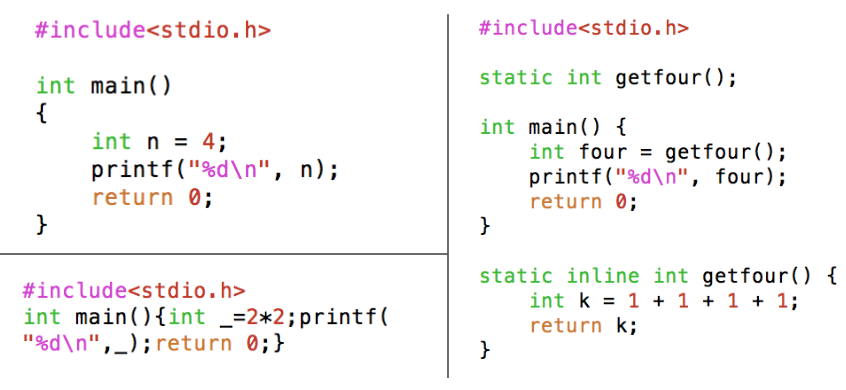
\includegraphics[width=0.5\textwidth]{3x4}
    \caption{Three different C programs that print the number 4 to stdout. When
    compiled with gcc's -O3 flag each program generates the same executable,
    verified by comparing MD5 hashes.}
    \label{fig:3x4}
\end{figure}

It has been shown in multiple studies that a programmer's code style is unique
within a limited population, such as a subset of students at RMIT University
\parencite{burrows2009application} or contestants in the Google Code Jam
programming competition \parencite{caliskan2015anonymizing}. Moreover, unique
code style can be used to reliably identify programmers from their source code
alone.  Caliskan-Islam et al. developed methods that could identify programmers
from 1600 candidates with 93\% accuracy in the above study. As seen in figure
\ref{fig:id-ml}, identifying authors from their source code is essentially a
machine learning problem.

\begin{figure}[!htb]
    \centering
    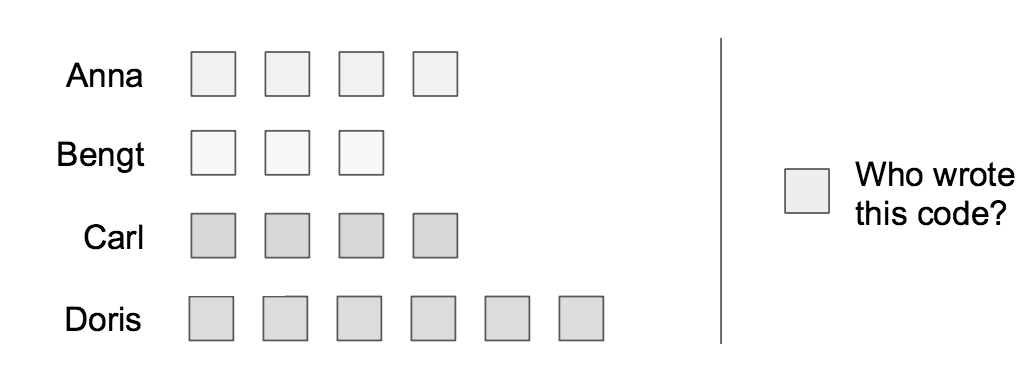
\includegraphics[width=0.5\textwidth]{id-ml}
    \caption{The problem of identifying programmers from their source code is
    essentially a machine learning problem: Given a \emph{training set} of
    source files with known authors, is it possible to ``learn'' the style of
    each author and accurately \emph{classify} a program outside of the
    training set? This is called the \emph{author classification problem}. }
    \label{fig:id-ml}
\end{figure}

Is the author classification problem solvable if, instead of their source code,
we only had access to the programmers' compiled executables? On face value it
is not at all clear that the necessary stylistic information survives the
compilation process; indeed, the three programs in figure \ref{fig:3x4} would
be impossible to differentiate because they all produce the exact same
executable when compiled. Nevertheless, in 2011 Rosenblum et al. developed
methods that could identify programmers from their compiled executables 
with 77\% accuracy from a set of 20 Google Code Jam contestants
\parencite{rosenblum2011wrote}, showing that the author classification problem
for compiled executables is in fact solvable in at least some cases. These
methods were improved upon by Caliskan-Islam et al. in 2015, achieving 96\%
accuracy in a similar dataset \parencite{caliskan2015coding}. 

Instead of trying to further improve upon the results of Caliskan-Islam et al.,
this thesis takes the opposite approach and examines what programmers can do to
\emph{prevent} de-anonymisation with the above methods. Specifically, we
examine how the methods of Rosenblum et al. \parencite{rosenblum2011wrote}
perform when the training data is compiled with various levels of compiler
optimisation (-O1 to -O3) turned on, as well as studying the effects of
statically linking the programs in the training data. This is something that
has not been examined in previous research.

\section{Problem statement}
The aim of this thesis is to investigate techniques that reduce the accuracy of
models in the author classification problem for compiled executables. We choose
an experimental approach and base our analysis around the methods proposed by
Rosenblum et al. \parencite{rosenblum2011wrote} for mainly practical reasons
described in section \ref{sec:scope}. The specific techniques we choose to
evaluate are the enabling of different levels of compiler optimisation (-O0 to
-O3 using gcc) and statically linking when compiling the models' training
data. This is captured by the following problem statement: 

\begin{italicquotes}
How do compiler optimisations and static linkage affect the accuracy of the
author classification models presented in \parencite{rosenblum2011wrote}?
\end{italicquotes}

\section{Motivation}
Methods that solve the author classification problem for compiled executables
could potentially be useful in a number of fields such as malware analysis or
plagiarism detection. However, little research exists on the robustness of such
methods against active adversaries. Common anti-analysis techniques such as the
use of packers or virtualisation can add a prohibitive pre-processing step to
the classification process \parencite{caliskan2015coding}, but the existence of
a truly non-reversible procedure for obfuscating the identifying features of a
program is an open research question. Investigating methods that can reliably
weaken the accuracy of classifiers in the literature is an important first
step to understanding how a more general solution could be constructed, if it
is in fact feasible at all.

From a programmer's point of view there are also a number of legitimate reasons
why one would want to remain anonymous. It could be that one's association with
the software could put them in danger (for example, a programmer that writes
anti-surveillance software in an oppressive state). It could also be the case
that the programmer simply does not want to be publicly associated with the
software. In this regard, it is highly desirable to give programmers the choice
of anonymity. Again, weakening the accuracy of classifiers in the literature is
an important first step towards this goal.

\section{Scope}
\label{sec:scope}
This thesis bases its analysis entirely around the methods presented by
Rosenblum et al. in \parencite{rosenblum2011wrote}. The reasons for doing so
are mainly practical; the programs used for feature extraction along with the
full dataset of features used in their study are available for download at the
authors' homepage. Having access to the same toolchain as the original authors
makes for a more reliable comparative study.

Analysis is limited to solutions from the 2010 round of the Google Code Jam
programming contest written in C++, one of the datasets used by Rosenblum et
al. Section \ref{sec:data-datasets} provides a more comprehensive description
of the datasets used.

\chapter{Background}
This section begins with an overview of the field. Moreover, the
technical concepts required to understand the rest of this thesis is introduced, and finally
the state-of-the-art in the field of authorship attribution is presented. Focus will
be on deriving authorship from binary programs; however, some related works
will be mentioned.

\section{Overview of the field}
Authorship classification belongs to a branch of computer science called
computer forensics. The goal of computer forensics is to analyse digital data
to obtain information, often in relation to computer crime
\parencite{reith2002examination}. In recent years machine learning techniques
have been used with great success to identify counterfeited integrated circuits
\parencite{huang2013counterfeit}, distinguishing different kinds of brain
tumours \parencite{zacharaki2009classification} and the automated detection of
software bugs \parencite{aleem2015comparative}, to name a few examples.

The first attempt at using statistical methods to de-anonymise programmers from
their code style was performed by Oman et al. \parencite{oman1989programming}
who classified programmers using a hand-picked, language-specific feature set.
In 2006, Frantzeskou et al. proposed a method using the analysis of byte level
n-grams (continuous sequences of n bytes) present in the source code which
greatly improved upon previous methods, along with being language-agnostic
\parencite{frantzeskou2006source}. In 2015, Caliskan-Islam et al. presented a
method based on features of the abstract syntax trees (ASTs) of C/C++ programs
that significantly improved the state-of-the-art again
\parencite{caliskan2015anonymizing}.
 
The 2011 study by Rosenblum et al. \parencite{rosenblum2011wrote} upon which this
thesis is based was first to show that author classification in compiled
executables is feasible. Features were extracted from the disassembled code and
the resulting control flow graph; this is explained in more detail in section
\ref{sec:feature-extraction}. In 2014 Alrabaee et al. improved upon the
accuracy of those techniques and proposed features that were more closely
related to programming style \parencite{alrabaee2014oba2}. In 2015,
Caliskan-Islam et al. further improved the state of the art using disassemblers
and decompilers, and applying their research in de-anonymising programmers from
source code to the ASTs of the decompiled binaries
\parencite{caliskan2015coding}. In the same report, Caliskan-Islam et al. also
perform a short side study on the effects of compiler optimisations have on
their methods, concluding that they result in a significant drop in accuracy
but not enough to be effective anonymisation tools. No other studies regarding
techniques for reducing the accuracy of classifiers for authorship attribution
in compiled executables were found.

\section{Technical Background}
This section includes the technical details necessary for understanding the
rest of this thesis. Initially it starts with a brief overview of the
compilation process and the static analysis. Moreover, this section describes
techniques used to extract features from binary executables and gives a short
explanation of support vector machines (SVMs) and their uses. 

A rudimentary understanding of the compilation process of C/C++ programs is
presumed, in particular the basic relationships between source code, assembly
code and binary machine code. Chapter 1 of \parencite{aho1986compilers}
provides a sufficient overview for the purposes of this thesis.

\subsection{Disassembly}
Disassembly is the task of generating a functionally equivalent assembly code
representation of a compiled executable. The general idea is to give a ``human
readable'' representation of a program that is easier to work with than the plain
binary data. Figure \ref{fig:disasm} shows a simple assembly routine, its
equivalent machine code after compilation and the resulting assembly code after
disassembly. Note that lexical data such as comments and whitespace do not
survive the compilation process.

\begin{figure}[!htb]
    \centering
    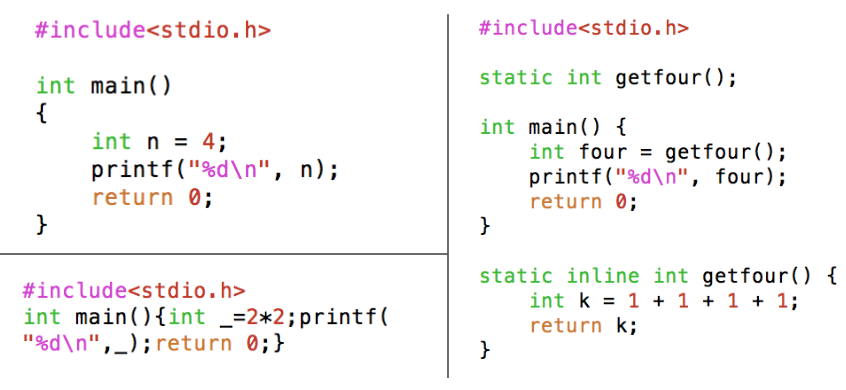
\includegraphics[width=0.5\textwidth]{3x4}
    \caption{TK: text and image}
    \label{fig:disasm}
\end{figure}

In general disassembly is a non-trivial task, especially with executables
targeting for complex instruction sets such as x86
\parencite{wartell2011differentiating}. Moreover, a number of techniques can be
employed to purposely thwart commonly used disassembly algorithms, making the
process much harder \parencite{linn2003obfuscation}. For the purpose of this
thesis, however, this is not an issue; the Dyninst library used for
disassembling (see section \ref{sec:feature-extraction} for details) is capable
of disassembling all compiled executables in the Google Code Jam dataset.

\subsection{Control flow analysis}
Control flow analysis of compiled executables is performed on assembly code
produced by a disassembler. The goal is to partition the code into so-called
``basic blocks'': sequences of instructions with exactly one entry point and
exit point with respect to program flow \parencite{allen1970control}. This
structure is captured in the control flow graph (CFG), a directed graph with
the basic blocks as nodes and control flow paths as edges. Figure
\ref{basic-blocks} illustrates the basic blocks of a simple assembly code
routine.

\begin{figure}[!htb]
    \centering
    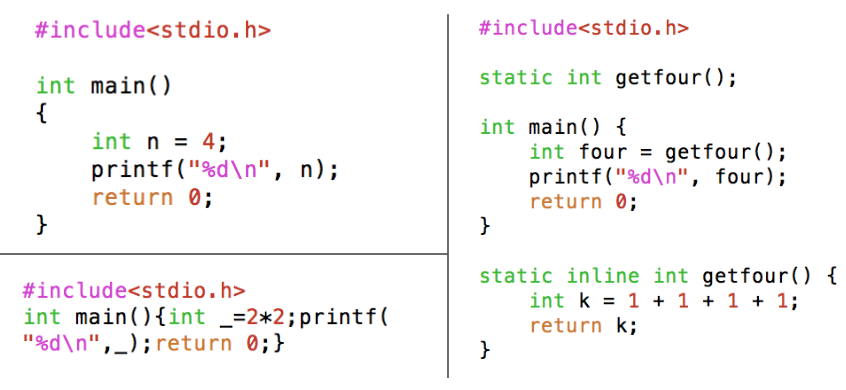
\includegraphics[width=0.5\textwidth]{3x4}
    \caption{TK: text and image}
    \label{fig:basic-blocks}
\end{figure}

The CFG provides a structured view of the binary at a higher level than
individual instructions. This can be used to identify high-level language
constructs such as loops and functions \parencite{cifuentes1993methodology} and
as such is used by decompilers such as the Hex-Rays decompiler (TK: Hex-Rays,
2016), used by Caliskan-Islam et al. in their paper improving on the work of
Rosenblum et al. \parencite{caliskan2015coding}. Rosenblum et al. also use the
CFG for feature extraction, but do not go as far as to decompile the binaries
\parencite{rosenblum2011wrote}.

\subsection{Derivatives of the CFG}
In their 2011 paper upon which this thesis is based, Rosenblum et al. defined
an additional two abstractions based on the CFG of a program: the
\emph{coloured control flow graph} (CCFG) and the \emph{coloured call graph}
(CCG).

The CCFG is a graph identical to the CFG with an additional \emph{colouring
function}. Each instruction in the target instruction set is classified as one
of fourteen instruction classes such as ``arithmetic instructions'' or
``branching instructions'', and a node's colour is simply a 14 bit bitmap
representing which instruction types are present in its corresponding basic
block. The colouring process is described in more detail in
\parencite{rosenblum2011recovering}, but further knowledge is not needed for
the rest of this thesis.

The CCG is created from the CFG by only including the subset of nodes that contain
a call instruction, with edges between two nodes representing a path between
the corresponding nodes in the original CFG. A colouring function is applied in
the same way as for the CCFG, with the colours depending on whether not the
node calls a library function, and if so, which library function is called.

\subsection{Support vector machines}
\label{sec:svms}
Support vector machines (SVMs) belong to a group of supervised learning methods
and are based on statistical learning theory. SVMs have been around since the
1960s and work well on for example text and image recognition. The learning
algorithm is given data and learns from that to identify patterns or classify
new data. There is a balance in how much data the algorithm should have. Using
too much information can lead to ``overfitting'' and the algorithm will perform
poorer for new data \parencite{cristianini2000introduction}. The goal is to
maximize the distance between data points in the different classes
 \parencite{awad2004effective}. 

\subsection{Mutual information}
When using SVMs for classification it is important to be weary of
``overfitting'' the training data, which can lead to poor predictive
performance \parencite{cristianini2000introduction}. A technique called
\emph{feature selection} can be used to prevent this from happening, the
general idea being to remove as many features as possible from the training
dataset until the model starts to lose predictive power. In order to decide
which features to remove first they must be ranked according to some criteria.
Mutual information (MI) is one such criteria \parencite{guyon2003introduction}.

In the case of the author classification problem, ranking is performed as
follows. Let $X$ be the multiset of all features generated for a given data
set. For all $x_i \in supp X$, let $P(X = x_i)$ denote the observed frequency
of $x_i$ in $X$. Likewise, let $Y$ be the set of all author labels and $P(Y =
y)= \frac{1}{|Y|}$ be the observed frequency of the label $y$ in $Y$ and let
$P(X=x_i,Y=y)$ denote the joint frequency of $x_i$ and $y$ in the data set.
Each unique feature $x_i \in supp X $ is ranked using the mutual information
criteria $R(x_i)$ \parencite{guyon2003introduction} in the following way:

$$R(x_i)= \sum_{x_i \in X, y \in Y} P(X=x_i,Y=y) \log \frac{P(X = x_i,
Y = y)}{P(X = x_i)P(Y = y)}$$

Intuitively the highly ranked features will be unique to a small set of 
labels in the training data and as such more useful in the classification
process, whereas the lowest ranked features can be removed without negatively
affecting the predictive power of the model. Removing superfluous features also
has the added benefit of reducing the time needed to train the model, which can
be important when working with high-dimensional data
\parencite{guyon2003introduction}.

\subsection{Cross-validation}
Cross-validation is a common method used when testing predictions. It is a
model used to analyze how well a predictive model will work in practice. When
using 10-fold cross-validation the data is randomly divided into 10 equally
sized sets, 9 of the sets is used for training and the remaining set is used
for the testing. This is repeated for each one of the sets, finally resulting
in an average measure of accuracy \parencite{hsu2003practical}.        

\section{State-of-the-art analysis}
As previously discussed, there are as far as we are aware of exactly three
papers presenting novel techniques to de-anonymise programmers from compiled
binary programs: \parencite{rosenblum2011wrote}, \parencite{alrabaee2014oba2}
and \parencite{caliskan2015coding}. In this section each approach will be discussed.
The focus will be on the techniques used by Rosenblum et al.

\subsection{Rosenblum et al.}
Rosenblum et al. evaluate their data on both a private dataset obtained from
an operating systems course (CS537) at the University of Wisconsin and a subset
of correct solutions from the 2009 and 2010 rounds of the Google Code Jam
(GCJ), specifically the solutions that:

\begin{itemize}
\item Were written in C/C++
\item Could be compiled using GCC 4.5 
\item Were submitted by an author that had submitted correct solutions to at
      least 8 problems in total
\end{itemize}

%TK: This thesis only care about 2010 data
In total, the GCJ dataset consisted of 2581 binaries (1,747 binaries from
2010) from 284 authors. Using 10-fold cross-validation on a set of 191 authors
from 2010, 51\% accuracy was achieved with 1900 features. For a randomly selected subset of 10
authors, 81\% accuracy was achieved and for a randomly selected subset of 20
authors 77\% accuracy.

\subsection{Alrabaee et al.}
Another study by Alrabaee et al. (An Onion approach to Binary code Authorship
Attribution) used an approach they called OBA2 to identify author style in
binary code \parencite{alrabaee2014oba2}. The study refers to the work of
Rosenblum et al. and argues that some of the features used in Rosenblum et al.
do not represent author style features. The result of the study
shows a higher accuracy than \parencite{rosenblum2011wrote}.The data used in
the study was the same as Rosenblum et al. 

\subsection{Caliskan-Islam et al.}
Another report published in December 2015 by Caliskan-Islam et al. improves on
the work of Rosenblum. This study has been able to improve author
identification accuracy even further also using data from Google Code Jam and
c/c++ binary code. With a set of 20 authors they are able to find the correct
author with 96\% accuracy. Caliskan-Islam (2015) also tested the effect of
different optimisations and got with 100 authors and no optimisation 78.3\%
accuracy and with level 3 optimisation 60.1\% accuracy. Furthermore, the study
found that it was easier to identify more experienced programmers.

\chapter{Method} \label{ch:method}
\section{Data and datasets} \label{data-datasets}
The analysis is based on data collected from the 2010 round of Google Code Jam
(GCJ). Specifically, the analysis is restricted to authors that have submitted at
least 8 submissions in C++. Furthermore, it is also required that solutions consist of exactly
one file with the extension .cpp which can be compiled and statically linked
with g++ in the test environment used (see section 3.2 for details).

Three subsets with 20, 191, and all 413 authors of the GCJ 2010 dataset are
used in order to test how the size of training data affects our analysis.
Furthermore, analysis on binaries compiled with the -static flag is
computationally infeasible with large datasets in our test environments. This
is summarised in Table~\ref{tab:datasets-summary}.

\begin{table}[!htb]
    \centering
        \begin{tabular}{ l l l }
        Authors & Subsets & Compiler flags \\ \hline
        413 & 413, 20 &  \lstinline{-O0, -O1, -O2, -O3} \\ 
        191 & 191, 20, 10 &  \lstinline{-O0, -O3} \\ 
        20 & 20, 10 &  \lstinline{-O0 static} 
        \end{tabular}
    \caption{Summary of subsets of the 2010 GCJ dataset used in our analysis}
    \label{tab:datasets-summary}
\end{table}

These dataset is chosen primarily to allow us to easily compare our results
with the existing literature; however, it should be said that the structure of
the GCJ dataset is a good fit for our analysis nonetheless. An
unsupervised classification algorithm is used with a large number of features; thus, it is
important to choose features derived from the coding style of the programmer
and not the problem itself. The GCJ dataset facilitates this since all
contestants solve the same set of problems; features derived from the problem
formulation perform poorly as classifiers and can be identified and discarded.
Likewise, features derived from the compilation process itself can also be
identified and discarded due to all solutions being compiled in the same way.

\section{Test environment}
All processing was done on an server running Fedora 23 x64.
Table~\ref{tab:dnf-packages} lists the dnf packages used in our test
environment that are not included in the base installation:

\begin{table}[!htb]
    \centering
        \begin{tabular}{ l l l }
        Package name & Version & Usage \\ \hline
        gcc-c++ & 5.3.1-2.fc23 & Compiling GCJ submissions \\
        python & 2.7.10-8.fc23 & Scripting, data manipulation \\
        libsvm & 3.20-5.fc23  & Support vector machine library \\
        libsvm-python & 3.20-5.fc23 & Python bindings for libsvm
        % TK: This is incomplete
        \end{tabular}
    \caption{\lstinline{dnf} packages not including in the base Fedora 23 x64
    installation that are used in our analysis}
    \label{tab:dnf-packages}
\end{table}

In a supplement to their 2011 paper, Rosenblum et al. provided the programs
they created for binary feature extraction as open source software. The same programs are used for our own analysis, albeit with minor changes due to
outdated dependencies\footnote{
    The original feature extraction source code can be found at
    \url{http://pages.cs.wisc.edu/~nater/esorics-supp/}. Our modified versions
    can be found at \url{https://github.com/macaullyjames/esorics}, along with
    installation instructions.
}.

\section{Feature extraction}
\label{sec:feature-extraction}
Feature extraction is the process of extracting measurable properties from the
sample dataset for further analysis. This section aims to provide a short
account of the \emph{feature templates} used by Rosenblum et al., on which this
thesis is based upon. For an in-depth account of how each feature template contributes
to the overall analysis, we refer to their original paper
\parencite{rosenblum2011wrote}.

Because it is not known which properties of the compiled binaries are
meaningful for determining authorship, the approach of Rosenblum et al. is to
extract a large number of generic features in the hope that authorship
information will be captured indirectly. All features are derived from the
program's disassembled code, coloured control flow graph (CCFG) and coloured
call graph (CCG) (section \ref{static-analysis-tb} explains these concepts in
detail) and are based on 6 feature templates: 

\begin{description}[style=nextline]
\item[Idioms]
All sequences of 1-3 instructions are extracted and counted from the
disassembled code. This is performed intraprocedurally; only sequences of
instructions within the same procedure are considered. Wildcard instructions
are allowed in order to capture more general instruction patterns.

\item[N-grams]
N-grams (continuous sequences of bytes) of length 3 or 4 are extracted from
the program. Again, this is performed intraprocedurally so n-grams outside of
procedures will be ignored.

\item[Graphlets]
All connected components of size 3 of the CCFG are extracted.

\item[Supergraphlets]
Each node in the CCFG is collapsed with a random neighbour and all connected
components of size 3 of the resulting graph are extracted. The algorithm used
to collapse nodes is described in detail in \parencite{rosenblum2011recovering} 

\item[Call graphlets]
All connected components of size 3 of the CCG are extracted.

\item[External interaction]
The name of each library routine used by the program is extracted.
\end{description}

Features are extracted for each program in the dataset and the set of unique
features in the entire dataset is generated; each feature can then be indexed
and recognised across programs. Finally, features are grouped by author and
saved in the LibSVM format \parencite{chang2011libsvm}
for analysis. 

\section{Feature selection}
The feature extraction process yields a high dimensional dataset with hundreds
of thousands to hundreds of millions of features. In order to speed up the
training of the SVM and avoid overfitting it is desirable to remove features
that provide little or no information about the authors’ programming style.
This is called \emph{feature selection}. Features are ranked with the mutual
information criteria presented in section \ref{sec:mi}, after which models are
trained with varying sizes of subsets of the highest ranking features. The
predictive power of each model is then evaluated (see section
\ref{sec:classification}) and the model that performs the best is retained.

Subset sizes of between 800 and 100000 are evaluated in all datasets. Models
trained with all features are also evaluated where doing so is computationally
feasible, however they consistently perform worse than models trained on
smaller subsets.

\section{Author classification}
As in the original paper from Rosenblum et al., classification is performed
using a linear support vector machine (SVM) \parencite{rosenblum2011wrote}. See
section 2.TK for details. The svm-scale program from the LIBSVM toolkit is used
\parencite{chang2011libsvm} to scale the feature values (avoids overweighting
frequently occurring features) to the interval [0, 1]:
\begin{lstlisting}
svm-scale -l 0 -u 1 features.dat > features.scale
\end{lstlisting}

The LIBLINEAR SVM implementation is then used \parencite{fan2008liblinear} for
training and evaluating via 10-fold cross-validation:
\begin{lstlisting}
train -v 10 features.scale
\end{lstlisting}


\chapter{Results}
As stated in the introduction, the aim of this thesis is to:
\begin{itemize}
\item Validate the results of \parencite{rosenblum2011wrote} on the 2010 Google
      Code Jam dataset
\item Investigate how g++’s optimisation flags (O1-O3) affect the accuracy of
      the author classification algorithm on the 2010 GCJ dataset
\item Investigate how statically linking the standard library affects the
      accuracy of the author classification algorithm on the 2010 GCJ dataset.
\end{itemize}

This section presents our results in each of these areas. On a similar 2010 GCJ
dataset used in \parencite{rosenblum2011wrote} our model performs comparably,
validating the results of Rosenblum et al. Compiler optimisations decrease the
predictive power of the model in all datasets and statically linked programs
are significantly harder to classify accurately. An in depth description of
each result follows.

\section{Validation of \parencite{rosenblum2011wrote}}
The 191 author subset described in section \ref{data-datasets} is
compiled without additional compiler optimisations (-O0). Our model is then
evaluated usng 10-fold cross-validation on each dataset using a varying number
of features, as described in chapter \ref{ch:method}. Additionally, we evaluate
our model using 20 randomly selected subsets of 20 authors in the same way.

In the 191 author subset we achieve at most 41.8\% accuracy. Rosenblum et al.
achieve 51\% accuracy in their comparable 191 author dataset. The chance of
randomly choosing the correct author among 191 candidates is 0.5\%.

In the 20 randomly selected subsets of 20 authors we achieve an average best
accuracy of 71.2\% with a standard deviation of 6.18\%. Rosenblum et al.
achieve an average 76.8\% accuracy in their comparable study of 20 random
subsets of 20 authors. The chance of randomly choosing the correct author
among 20 candidates is 5\%

While our models do not perform quite as well as those of Rosenblum et al.,  we
argue that the difference in accuracy is reasonable and also expected. This is
discussed further in section TK. In both datasets our model performs
significantly better than chance and as such the general approach of Rosenblum
et al. seems to be valid.

Figure TK summarises our results compared to that of Rosenblum et al.

\section{Optimisation levels -O1 to -O3}
The full 413 author dataset is compiled with optimisation levels -O1 to -O3 and
compared to a baseline dataset compiled without additional compiler
optimisations enabled (-O0). Compiler optimisations lead to an increase in both
unique features and the total number of features extracted from the programs,
the -O3 dataset yielding 5 times the number of unique features as the -O0
dataset and a 63\% increase in the total number of features. Models trained on
the -O1 and -O2 datasets do not perform significantly worse than the baseline
(28.6\%, 27.6\%  vs 32.5\%) whereas the -O3 dataset yields an accuracy of just 21.6\%.
This is summarised in table \ref{tab:413-results}.

\begin{table}[!htb]
    \centering
        \begin{tabular}{ l l l l }
        Optimisation level & Model accuracy \\
        \hline
        \lstinline{-O0} & 32.5\% \\
        \lstinline{-O1} & 28.6\% \\
        \lstinline{-O2} & 27.6\% \\
        \lstinline{-O3} & 21.6\%
        \end{tabular}
    \caption{How accuracy varies depending on optimisation level in the full
    413 author dataset}
    \label{tab:413-results}
\end{table}

Interestingly, the number of features selected by cross-validation is roughly
the same for all optimisation levels. This despite that both the number of
unique features and total number of features vary greatly, as seen in table
\ref{tab:413-results-features}.

\begin{table}[!htb]
    \centering
        \begin{tabular}{ l l l l }
        Optimisation level & Unique & Total & Selected \\ \hline
        \lstinline{-O0} & 765307 & 13204201 & 7000 \\
        \lstinline{-O1} & 2141558 & 15532246 & 9000 \\
        \lstinline{-O2} & 2593340 & 16681152 & 10000 \\
        \lstinline{-O3} & 3891494 & 21570182 & 10000
        \end{tabular}
    \caption{The number of unique features, total number of features and number
    of features selected by cross-validation for each optimisation level in the
    full 413 author dataset}
    \label{tab:413-results-features}
\end{table}

The same analysis is performed on 20 random subsets of 20 authors from the same
413 author dataset. Again, models trained on the -O1 and -O2 subsets do not
perform significantly worse than the baseline on average (65.4\% and 64.4\%
vs 68.8\%, respectively) while the -O3 subsets yield an average accuracy of
58.7\%. This is summarised in table \ref{tab:20-results}.

\begin{table}[!htb]
    \centering
        \begin{tabular}{ l l l l }
        Optimisation level & Average accuracy & Standard deviance \\
        \hline
        \lstinline{-O0} & 68.8\% & 5.1\% \\
        \lstinline{-O1} & 65.4\% & 6.9\% \\
        \lstinline{-O2} & 64.4\% & 7.0\% \\
        \lstinline{-O3} & 58.7\% & 5.7\% 
        \end{tabular}
    \caption{Average accuracy and standard deviance per optimisation level for
    models over 20 random subsets of 20 authors from the full 413 author
    dataset.}
    \label{tab:20-results}
\end{table}

In summary, we find that the use of compiler optimisation flags does
consistently decrease the accuracy of our models, even though they still
perform significantly better than random chance. With the highest optimisation
level, -O3, a 10\% drop in accuracy is observed in both the full 413 author
dataset and random subsets of 20 authors.

\section{Statically linked programs}
A subset of 20 authors is compiled and statically linked with optimisation
level -O0. This is compared to a baseline dataset of the same 20 authors
compiled without additional optimisations (-O0) but dynamically linked. The
statically linked programs yield 3859605 unique features and 110725073 features
in total. In comparison, the baseline dataset yields 122420 unique features and
618918 features in total, meaning the statically linked programs yield more
than 30 times the number of unique features and almost 180 times the number of
features in total. Models trained on the statically linked programs also
performed considerably worse than the baseline: 28.6\% vs 75.0\%. The number of
features selected by cross-validation is roughly the same in both cases. These
results are summarised in table \ref{tab:20-static-results}.

\begin{table}[!htb]
    \centering
        \begin{tabular}{ l l l l l }
        Linkage & Model accuracy & Unique features & Total features &
        Selected features \\ \hline
        \lstinline{Dynamic} & 75.0\% & 122420 & 618918 & 7000 \\
        \lstinline{Static} & 28.6\% & 3859605 & 110725073 & 9000 \\
        \end{tabular}
    \caption{Comparison of model accuracy, number of unique features, total
    number of features and number of features selected by cross-validation for
    dynamically respectively statically linked programs from the same 20 author
    dataset} 
    \label{tab:20-static-results}
\end{table}

The same analysis is performed with 20 randomly selected subsets of 10 authors
from the 20 author dataset used above. Again, models trained on the statically
linked programs perform significantly worse than models trained on their
dynamially linked counterparts, as seen in table \ref{tab:10-static-results}. 

\begin{table}[!htb]
    \centering
        \begin{tabular}{ l l l }
        Linkage & Average accuracy & Standard deviance \\
        \hline
        Dynamic & 81.2\% & 7.3\% \\
        Static & 45.5\% & 6.6\%
        \end{tabular}
    \caption{Average accuracy and standard deviance for models over 20 random
    subsets of 10 authors with static and dynamic linkage, respectively}
    \label{tab:10-static-results}
\end{table}

We conclude that statically linking the programs in our dataset leads to a
large increase of unique features and total number of features, and
significantly reduces the accuracy of our models.

\chapter{Discussion}
\section{Method discussion}
When attempting to implement the method used in Rosenblum et al. it was not
without difficulties. To be able to use the source code provided by Rosenblum
et al. some adjustments to the source code had to be made, updating it to make
it work on a more modern system. As far as we can tell it has not caused any
errors.

The source code provided by Rosenblum et al. was only for feature extraction.
Therefore, it is possible that inconsistencies with the method of Rosenblum et al. could have
emerged from the process of converting output data from the feature extraction to
data with the LIBSVM format needed for LIBLINEAR.

Something to note is that a larger number of features than Rosenblum et al. was needed to achieve high
accuracy. One reason could be that our implementation of feature selection may differ from that of
Rosenblum et al. 

\section{Results analysis}
The experiments conducted show that optimisation reduces the accuracy. This is
similar to what \parencite{caliskan2015coding} found in their experiments. As
previously mentioned, they got with 100 authors and no optimisation 78.3\%
accuracy and with level 3 optimisation 60.1\% accuracy.

When optimisation is used to compile the binaries there tend to be a larger
amount of features extracted. Optimisation with -O3 gave 3891494 unique
features in the case with 413 authors compared to 736307 features when -O0 was
used. That is more than five times as many features. For optimisation -O3  the
highest accuracy with 20 authors was 58.66\% compared to 68.80\% when no
optimisation was used (see Figure 4.2. and Figure 4.8.), a 10.14\% difference).
Furthermore, optimisation with -O1 and -O2 gave only a small reduction in
accuracy. The results are still much higher than the random chance 5\% of
guessing the author . 

Experiments with subsets of 20 authors from the set of 191 authors shows
similar results. When no optimisation was used the highest accuracy was 71.22
\% compared to 59.79\% when -O3 was used (see Figure 4.X. and  Figure 4.X. ).
In this case the difference is 11.43\%.

It is also possible to see that the accuracy is higher when fewer authors is
used which is not that strange, random chance of guessing the correct author is
also higher 10\%. If the case with 20 authors and no optimisation from the set
of 191 is compared with that of 10 authors (see Figure 4.X.) the highest
accuracy with 10 authors and was 81.58\% compared to 71.22\% with 20 authors.
The difference is 10.36\%.

When using static with only 20 authors the unique number of features was
3859605 and the total number of features was 110725073. In contrast, even
though using more authors,  the number of unique features from the set of 191
authors was 509908 and the total number of features was only 6221646.The
accuracy achieved in the case using static linking and 10 authors was 45.54\%
compare to 81.58\%. Thus, an important factor affecting the accuracy seems to
be the number of features. 

Even though it was not possible to replicate Rosenblum’s et al. (2011) experiment and data
exactly, our experiments showed accuracy levels not far from theirs. Using 191
authors and 20 authors \parencite{rosenblum2011wrote} got approximately 77\% while
our experiment using 191 authors gave 71\%; however, with a different number of files and
probably not the exact set of 191 authors.     

With no optimisation and using all 191 authors and 7000 features an accuracy of
41.8\% was achieved (see Figure 4.23). It is much better than random chance
0.5\%. \parencite{rosenblum2011wrote} achieved 51\% on the full set with 191
authors using only 1900 features. Not only did they achieve better results,
they also manage to do this using fewer features. This could indicate that our
implementation of feature selection differ from that of Rosenblum et al.

\section{Future research}
There are more techniques one could use when processing the source code or the
binaries that could be interesting to investigate further. It would be
interesting to test how different packers affect the accuracy. Moreover, it
would be interesting to see how this method would work in more practical
situations. Is it possible to identify teams using these techniques? What if
the team’s members change frequently? What if two teams enforce the same style
guide? In real situations the source code could be processed using different methods.
What would happen if the binaries were compiled with a mix of different
optimisation levels and static?  

Most of the previous reports have focus on source code from the Google Code Jam
programming competition. More research on other datasets with larger files
could be interesting to examine.

With the purpose of testing the accuracy values obtained it could also be
interesting to use different machine learning approaches. Possible try another
program than LIBLINEAR for the cross-validation.

\chapter{Conclusion}
This thesis attempted to verify the authorship attribution method created by
\parencite{rosenblum2011wrote}. Our results tend to be somewhat lower than that
of Rosenblum et al. and need more features to give high accuracy; nevertheless,
the method seems to be working. Some possible explanations concerning the
differences in accuracy achieved could be because of difficulties in
implementing Rosenblum et al. method exactly. Furthermore, even though working
with data from Google Code Jam 2010 the exact dataset that Rosenblum et al.
used could not be replicated and therefore cause differences in results. 

Optimisation seems not be enough to make authors anonymous; however, it reduces
the accuracy somewhat. Adding static causes a bigger drop in accuracy. The
accuracy achieved in the case using static and 10 authors was 45.54\% compare
to 81.58\% without. Perhaps not enough to ensure anonymity; nevertheless,
static gives a significantly lower accuracy. The data extracted from the binaries shows that
optimisation and static linking results in more features that may be the cause
of the reduction in accuracy.

\printbibliography

\end{document}
